\subsection{Overview}
The TrackMe services are built on a client-server structure, this way the system is organized through abstraction levels.
We chose to adopt a 3-tier architecture.
\\[0.2cm]
\begin{figure}[H]
\centering
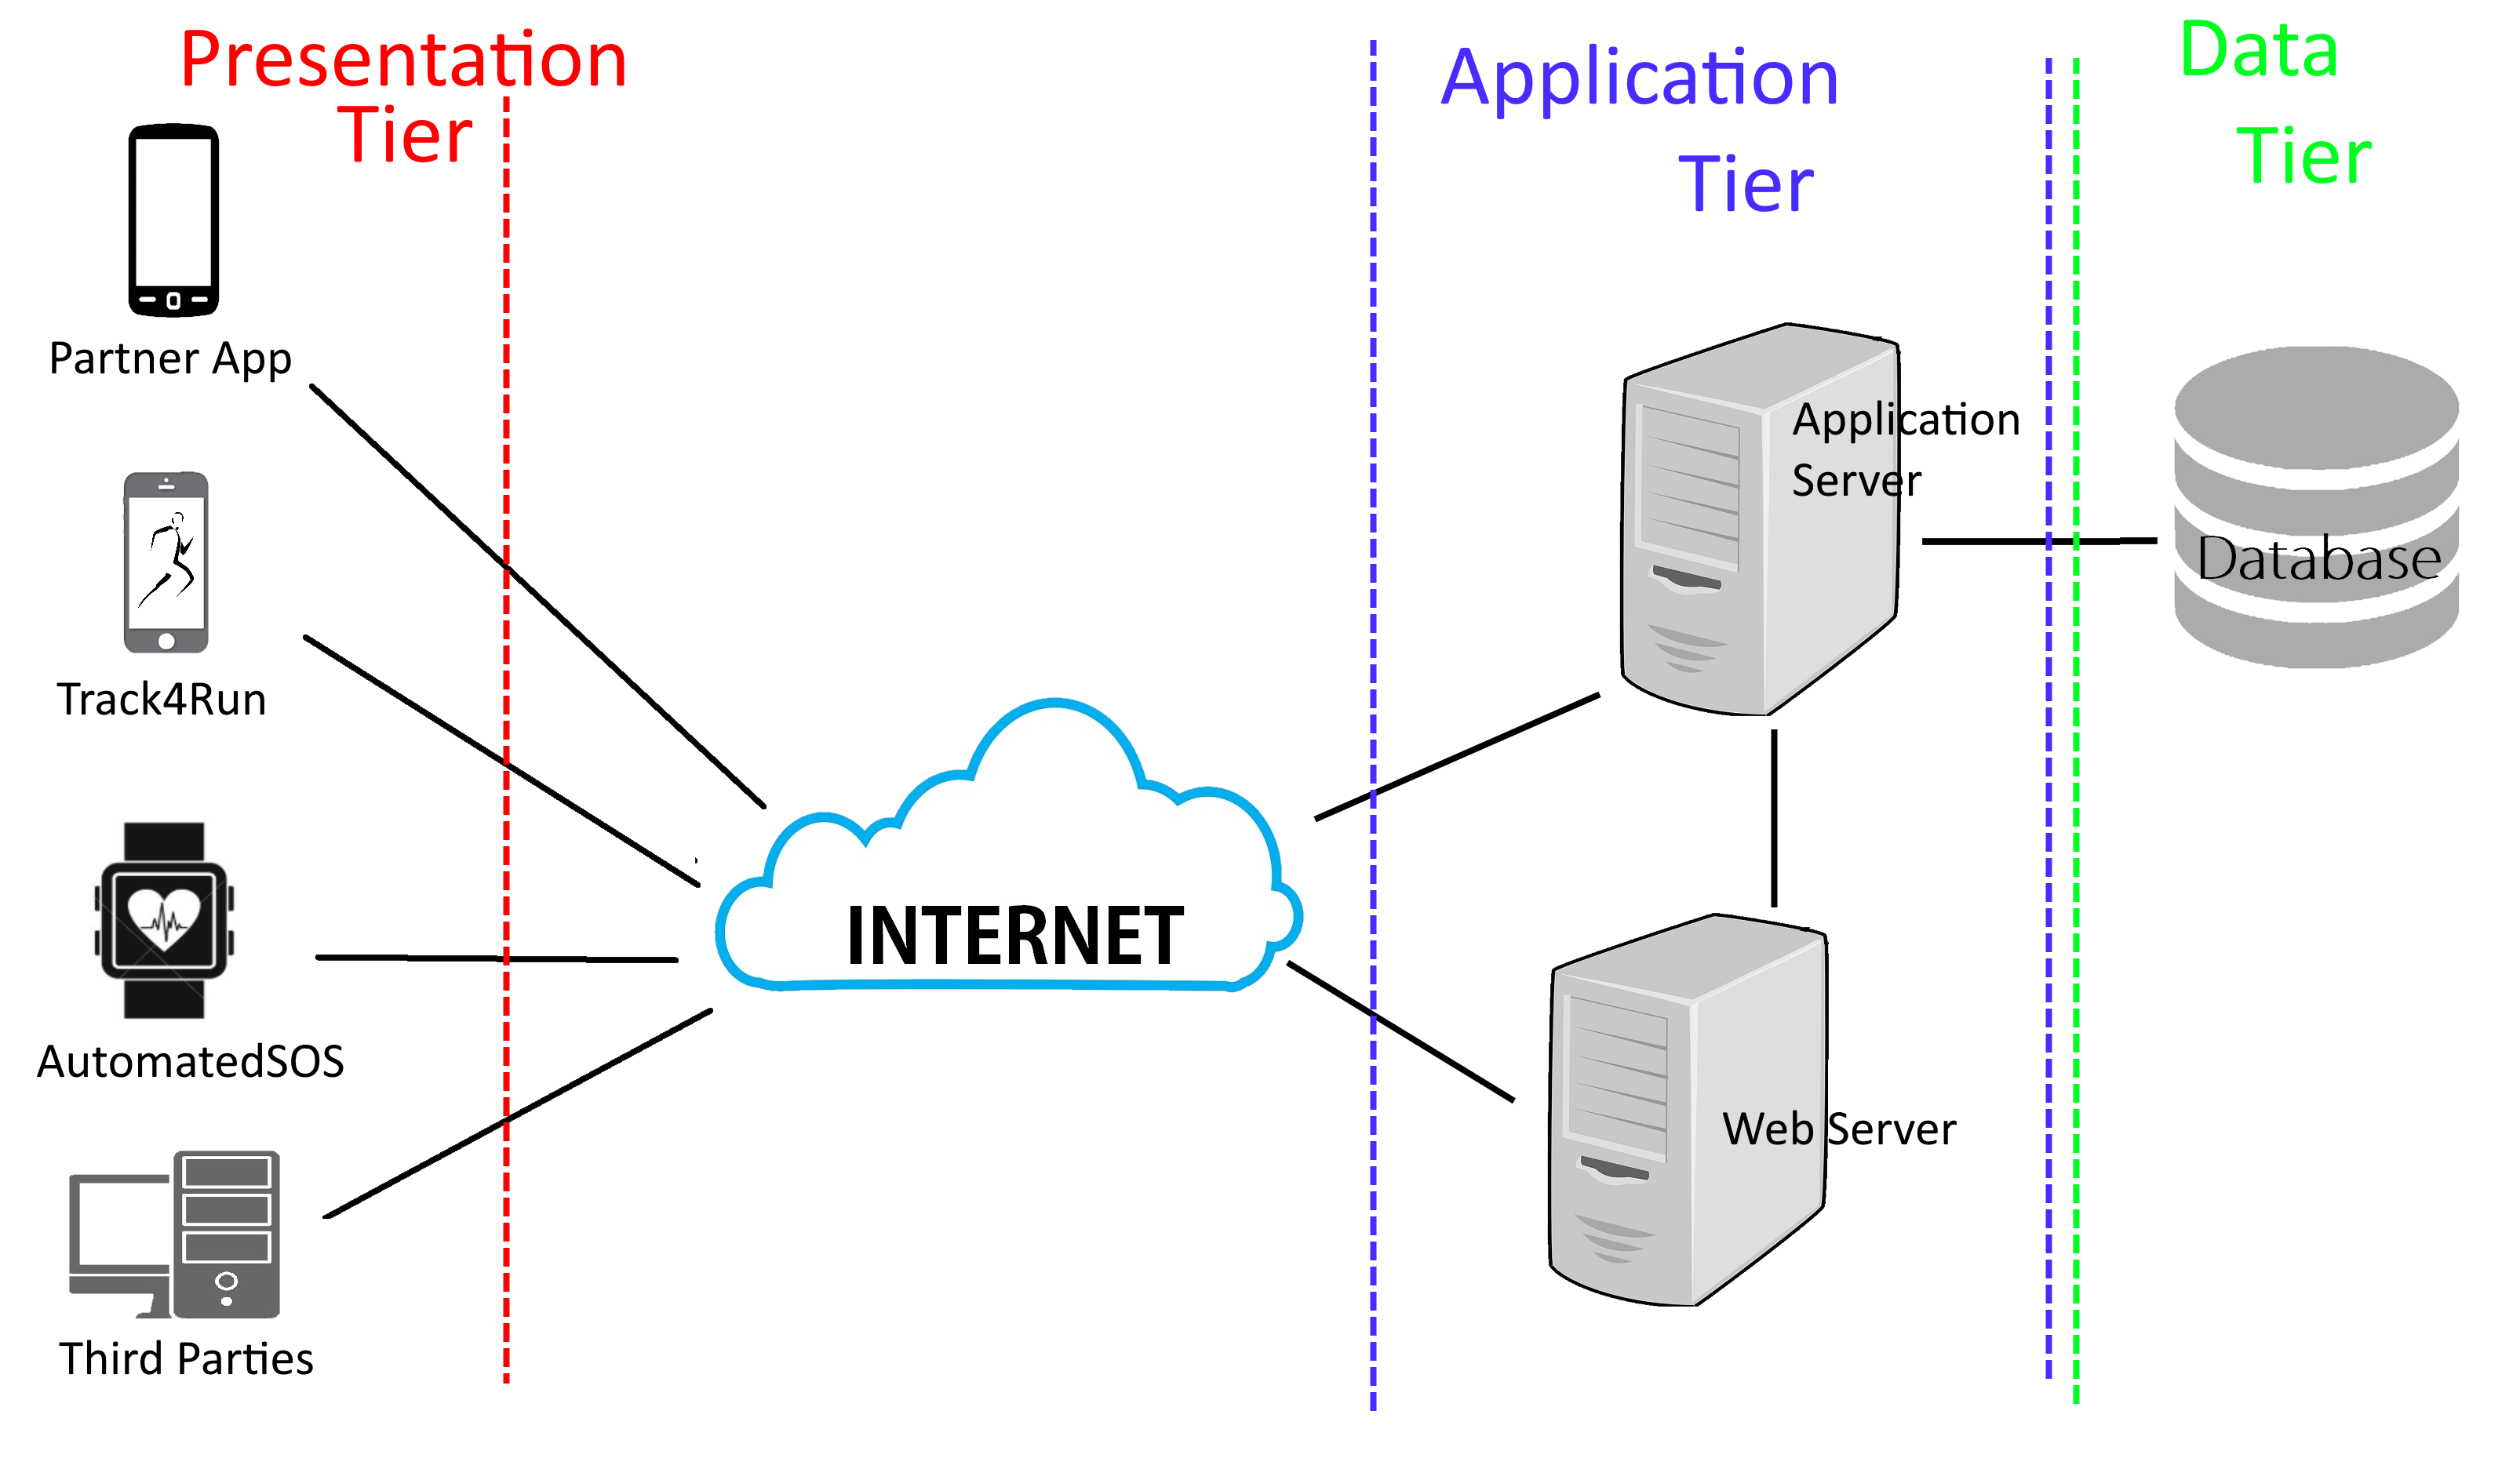
\includegraphics[scale=0.18]{Images/Overview.png}
\caption{Overview architecture }
\end{figure}

\begin{itemize}
	\item \textbf{Presentation Tier} \\This layer makes the interaction possible between the user and the system. Here, the user sees all the information provided by the system in an easy and understandable way. This layer regards both the interaction with third parties and individuals. 
	\item \textbf{Application Tier} \\This layer, managed almost totally by Data4Help service, is in charge of:
	\begin{itemize}
		\item storing into the database the users' data;
		\item collecting data from the database in order to answer to third parties' requests;
		\item generating statistics on collected data;
		\item sending requested data to third parties.
		\item managing run events, creating them and enrolling athletes to them.
	\end{itemize}
	Moreover, even AutomatedSOS has a part of the logic application in order to continuously monitor users' health status.
	\item \textbf{Data Tier} \\In this layer all the users' data (location and health status) are stored into the database and are retrieved by the application tier in order to do statistics and answer third parties' requests. In addition, information about the run events, third parties' and individuals' credentials are stored.
\end{itemize}
\bigbreak
\noindent
More precisely, Data4Help manages the data and the core system logic while AutomatedSOS and Track4Run manage the presentation section. Actually, as already said, a small part of application tier is also present in AutomatedSOS, this is due to the fact that the Health Monitoring process requires to be executed as fast as possible. 
\subsection{Component View}

\subsubsection{Component Diagram}
\begin{figure}[H]
\centering
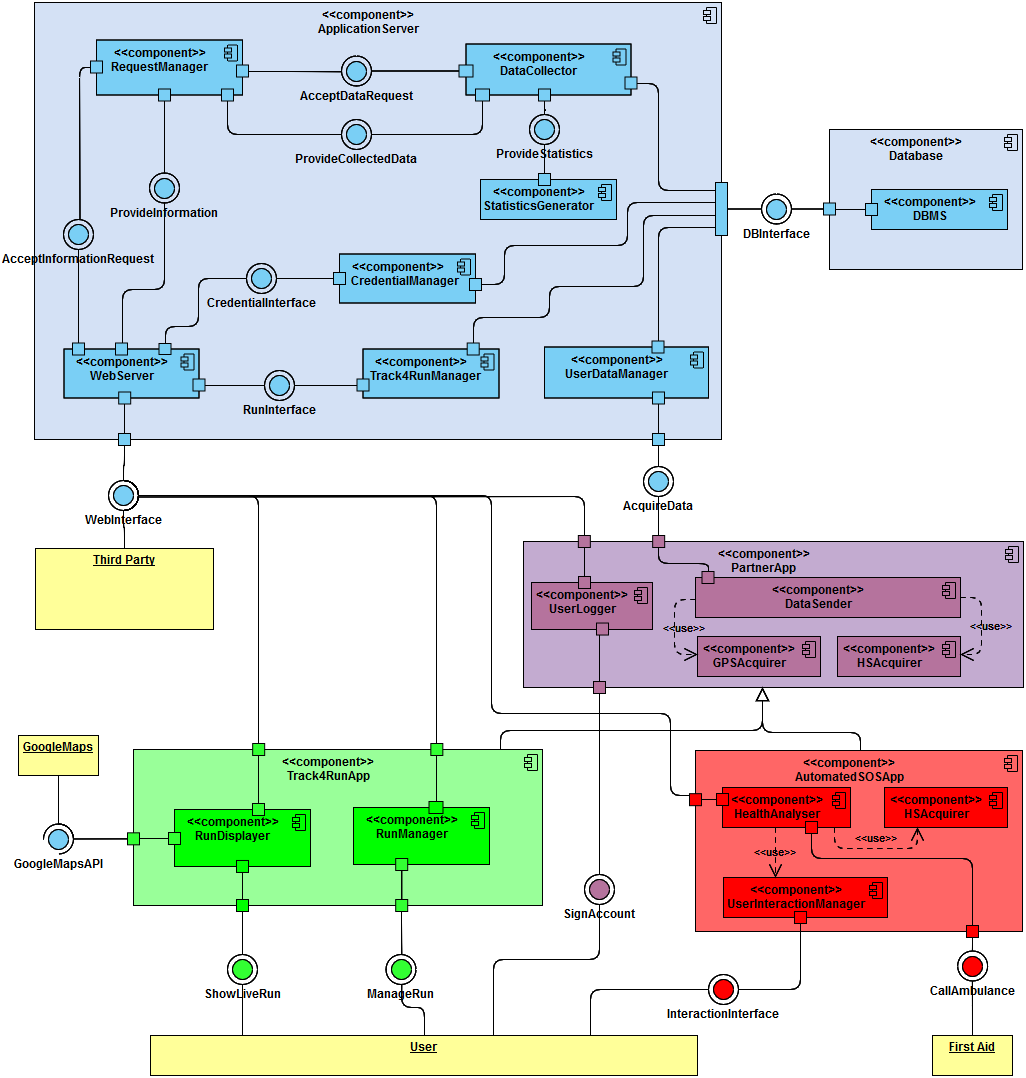
\includegraphics[scale=0.7]{Images/ComponentDiagram.png}
\caption{Component Diagram}
\end{figure}

{\large \textbf{Component diagram description}}
\begin{enumerate}
\item [1] \textbf{ApplicationServer} 
This large component is in charge of managing Data4Help services like storing and providing, for interested companies, users’ data such as GPS location and daily Health Status. Moreover it manages run information for Track4Run application.

	\begin{enumerate}
	\item [1.1] \textbf{WebServer:} In order to accept requests and supply information to whoever needs them, this component offer a friendly web interface to simplify these operations.
		
	\item [1.2] \textbf{RequestManager:} In order to support the web server in its job, this component manages all the incoming requests: it sorts them per urgency, it wraps the requests in a smart data structure and sends it to the DataCollector. Also it unwraps the answers from the Data Collector and it continuously generates data exchange if a live acquisition is active.
		
	\item [1.3] \textbf{DataCollector: } This component communicates with the Database in order to retrieve information and supply them to the RequestManager. In order to perform these operations whenever the DataCollector receives requests from the RequestManger, it unwraps them, creates a query and sends it to the Database; once the Database answered the query, the DataCollector should wrap the answer and provide it to the RequestManager. Moreover if statistics on data are needed the DataCollector also sends data to the StatisticsGenerator which will answer with the statistic of interest.
		
	\item [1.4] \textbf{StatisticsGenerator: } This component generates statistics on data provided by the DataCollector such as arithmetic mean, variance from average, standard deviation and median.

	\item [1.5] \textbf{UserManager: } This component communicates with users' device in order to store into the Database data automatically collected by applications.

	\item [1.6] \textbf{Track4RunManager: } This component communicates with the Track4Run application in order to store into the database all the information about promoted run events, all the lists of athletes participating to runs and so on.
	
	\item [1.7] \textbf{CredentialManager: } This component communicates with the WebServer in order sign up/in users to the system and to check whether the credentials inserted by a user that wants to log in are correct or not.
	
	\end{enumerate}
	
\item [2] \textbf{Database} 
This component is in charge of physically storing data and organize them in a smart way according to DBMS rule, moreover it allows the access to those data.

	\begin{enumerate}
	\item [2.1]\textbf{DBMS: }
	This component is in charge of storing all the data involving the system like users' parameters, third parties' requests and races' information generated by the Track4Run application.
	\end{enumerate}
	
\item [3]\textbf{PartnerApp: }
This component describes how the partner applications of TrackMe are structured, from the components in charge of retrieving raw data from the device's API, to the components in charge of communicating with the Main Server. The PartnerApp component is extended by all the partner applications that want to exploit Data4Halp service, so even by AutomatedSOS and Track4Run.

	\begin{enumerate}
	\item [3.1]\textbf{GPSAcquirer:}
	This component acquires the user's GPS location at constant time periods.
	
	\item [3.2]\textbf{HSAcquirer:}
	This component acquires hearth rate, blood pressure and calories consumed from user's device at constant time periods.
	
	\item [3.3]\textbf{UserLogger:}
	This component offers to the user the possibility to sign up/in. For this reason it is in charge of showing the data policy and acquiring all the credentials inserted during registration. Moreover it has to communicate with the WebServer in order to forward the sign up/in request.
	 
	\item [3.3]\textbf{DataSender:}
	This component exploits GPSAcquirer and HSAcquirer in order to provide to the UserManager component all the retrieved data.
	\end{enumerate}

\item [4]\textbf{AutomatedSOSApp: }
This component extends all that is specified in the PartnerApp component to exploit all its features. AutomatedSOS component has to use the HSAcquirer in order to check health status parameters and call the First Aid whenever it is required.

	\begin{enumerate}
	\item [4.1]\textbf{HealthAnalyser: }
	This component exploits HSAcquirer features in order to continuously analyze health parameters, compare the last acquired data with historical ones to improve the analyzing process, and last, it checks data in order to prevent user's diseases and call an ambulance whenever such parameters are below a certain threshold compiling and providing a special report to First Aid.
	
	\item [4.2]\textbf{HSAcquirer:}
	This component acquires hearth rate, blood pressure and calories consumed from user's device at constant time periods.
	
	\item [4.3]\textbf{UserInteractionManager:}
	This component gives to the user the possibilities to see his/her current or historical health status, to set preferences, and to get a feedback message whenever an ambulance has been sent to his/her location.
	\end{enumerate}
	

\item [5]\textbf{Track4RunApp: }
This component extends all that is specified in the PartnerApp component to exploit all its features. Track4Run component will also provide to users the possibility to select and spectate a run, allow promoters to create and manage a run and last allow athletes to enroll to a given run.
	
		\begin{enumerate}
	\item [5.1]\textbf{RunDisplayer: }
	 This internal component is in charge of providing a human interface to the user that allows him to specify the run he wants to spectate and then shows the position of all the athletes in that particular run exploiting GoogleMapsAPI.
	
	\item [5.2]\textbf{RunManager: }
	This internal component provides to the user the possibility to promote a run specifying fields like date, path, name, maximum number of participants and description. Moreover a promoter can invite specific athletes providing their fiscal code. 
	\end{enumerate}

\end{enumerate}

\clearpage

\subsubsection{Entity Relationship Diagram}
The following figure shows how data are stored inside the database using an Entity Relationship Diagram.
\begin{figure}[H]
\centering
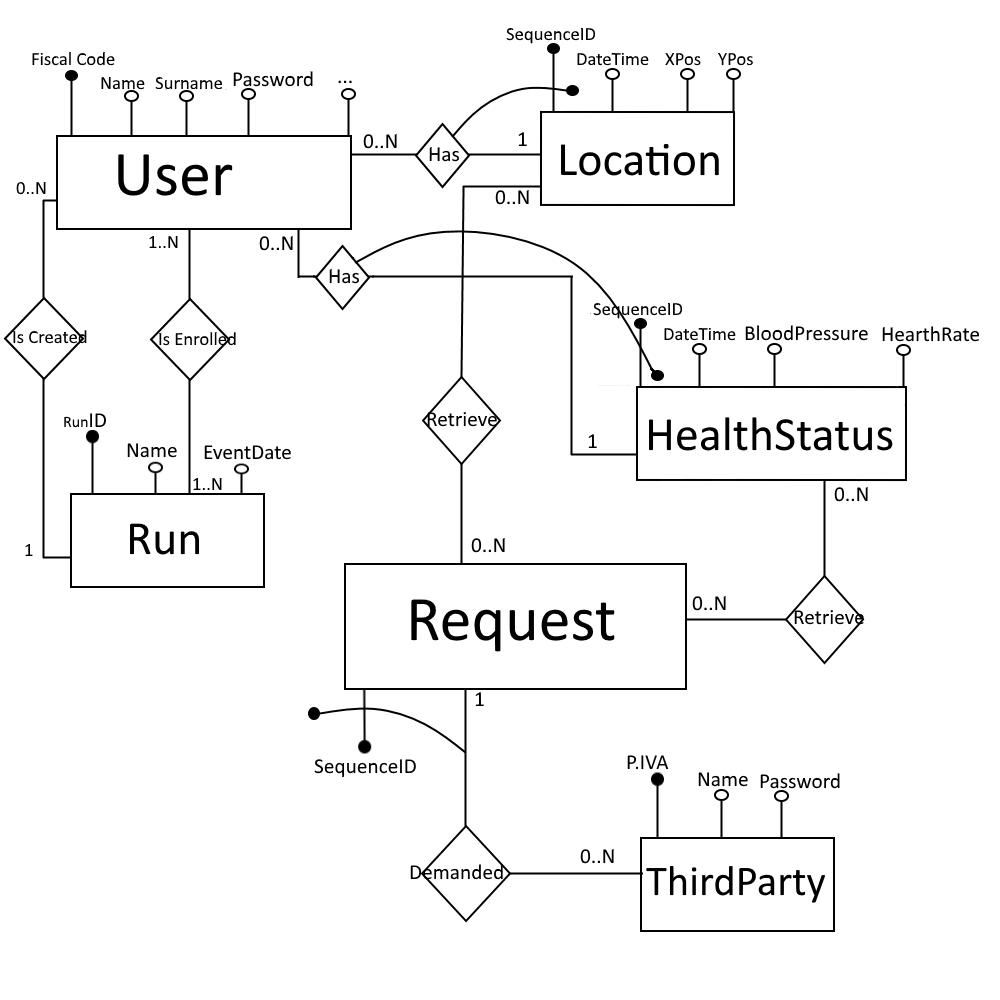
\includegraphics[scale=0.65]{Images/ERDiagram.png}
\caption{Entity Relationship Diagram Diagram}
\end{figure}
\noindent
This diagram explains how for each user subscribed to Data4Help system are associated several data in order to create an history of his/her movements (Location) and health parameters (Health Status). In the diagram all the third parties and their requests done are also stored. Moreover, all the informations about the run for Track4Run application (including promoter, enrollers, event date etc.) are stored.

\newpage
\subsection{Deployment View}
The following Deployment Diagram captures the topology of the system's hardware and software distribution.
\bigbreak
\noindent
The SmartphoneApp, the SmartwatchApp and WebBrowser communicate to the WebServer through HTTP protocol due to the fact that the applications are based on browsers in order to improve portability among different Operative Systems. The two applications also communicate directly to the Application Server in order to exchange automatically retrieved data like the GPS Location and the Health Status.
\bigbreak
\noindent
The WebServer runs on a RedHat system on which Java Servlets and JSPs are deployed, also it communicates to the Application Server through RMI.
\bigbreak
\noindent
The Application Server runs on an Ubuntu system on which the business logic  of the system is deployed, also it communicates to the DB Server through JDBC.
\vspace{1.0 cm}

\begin{figure}[H]
\centering
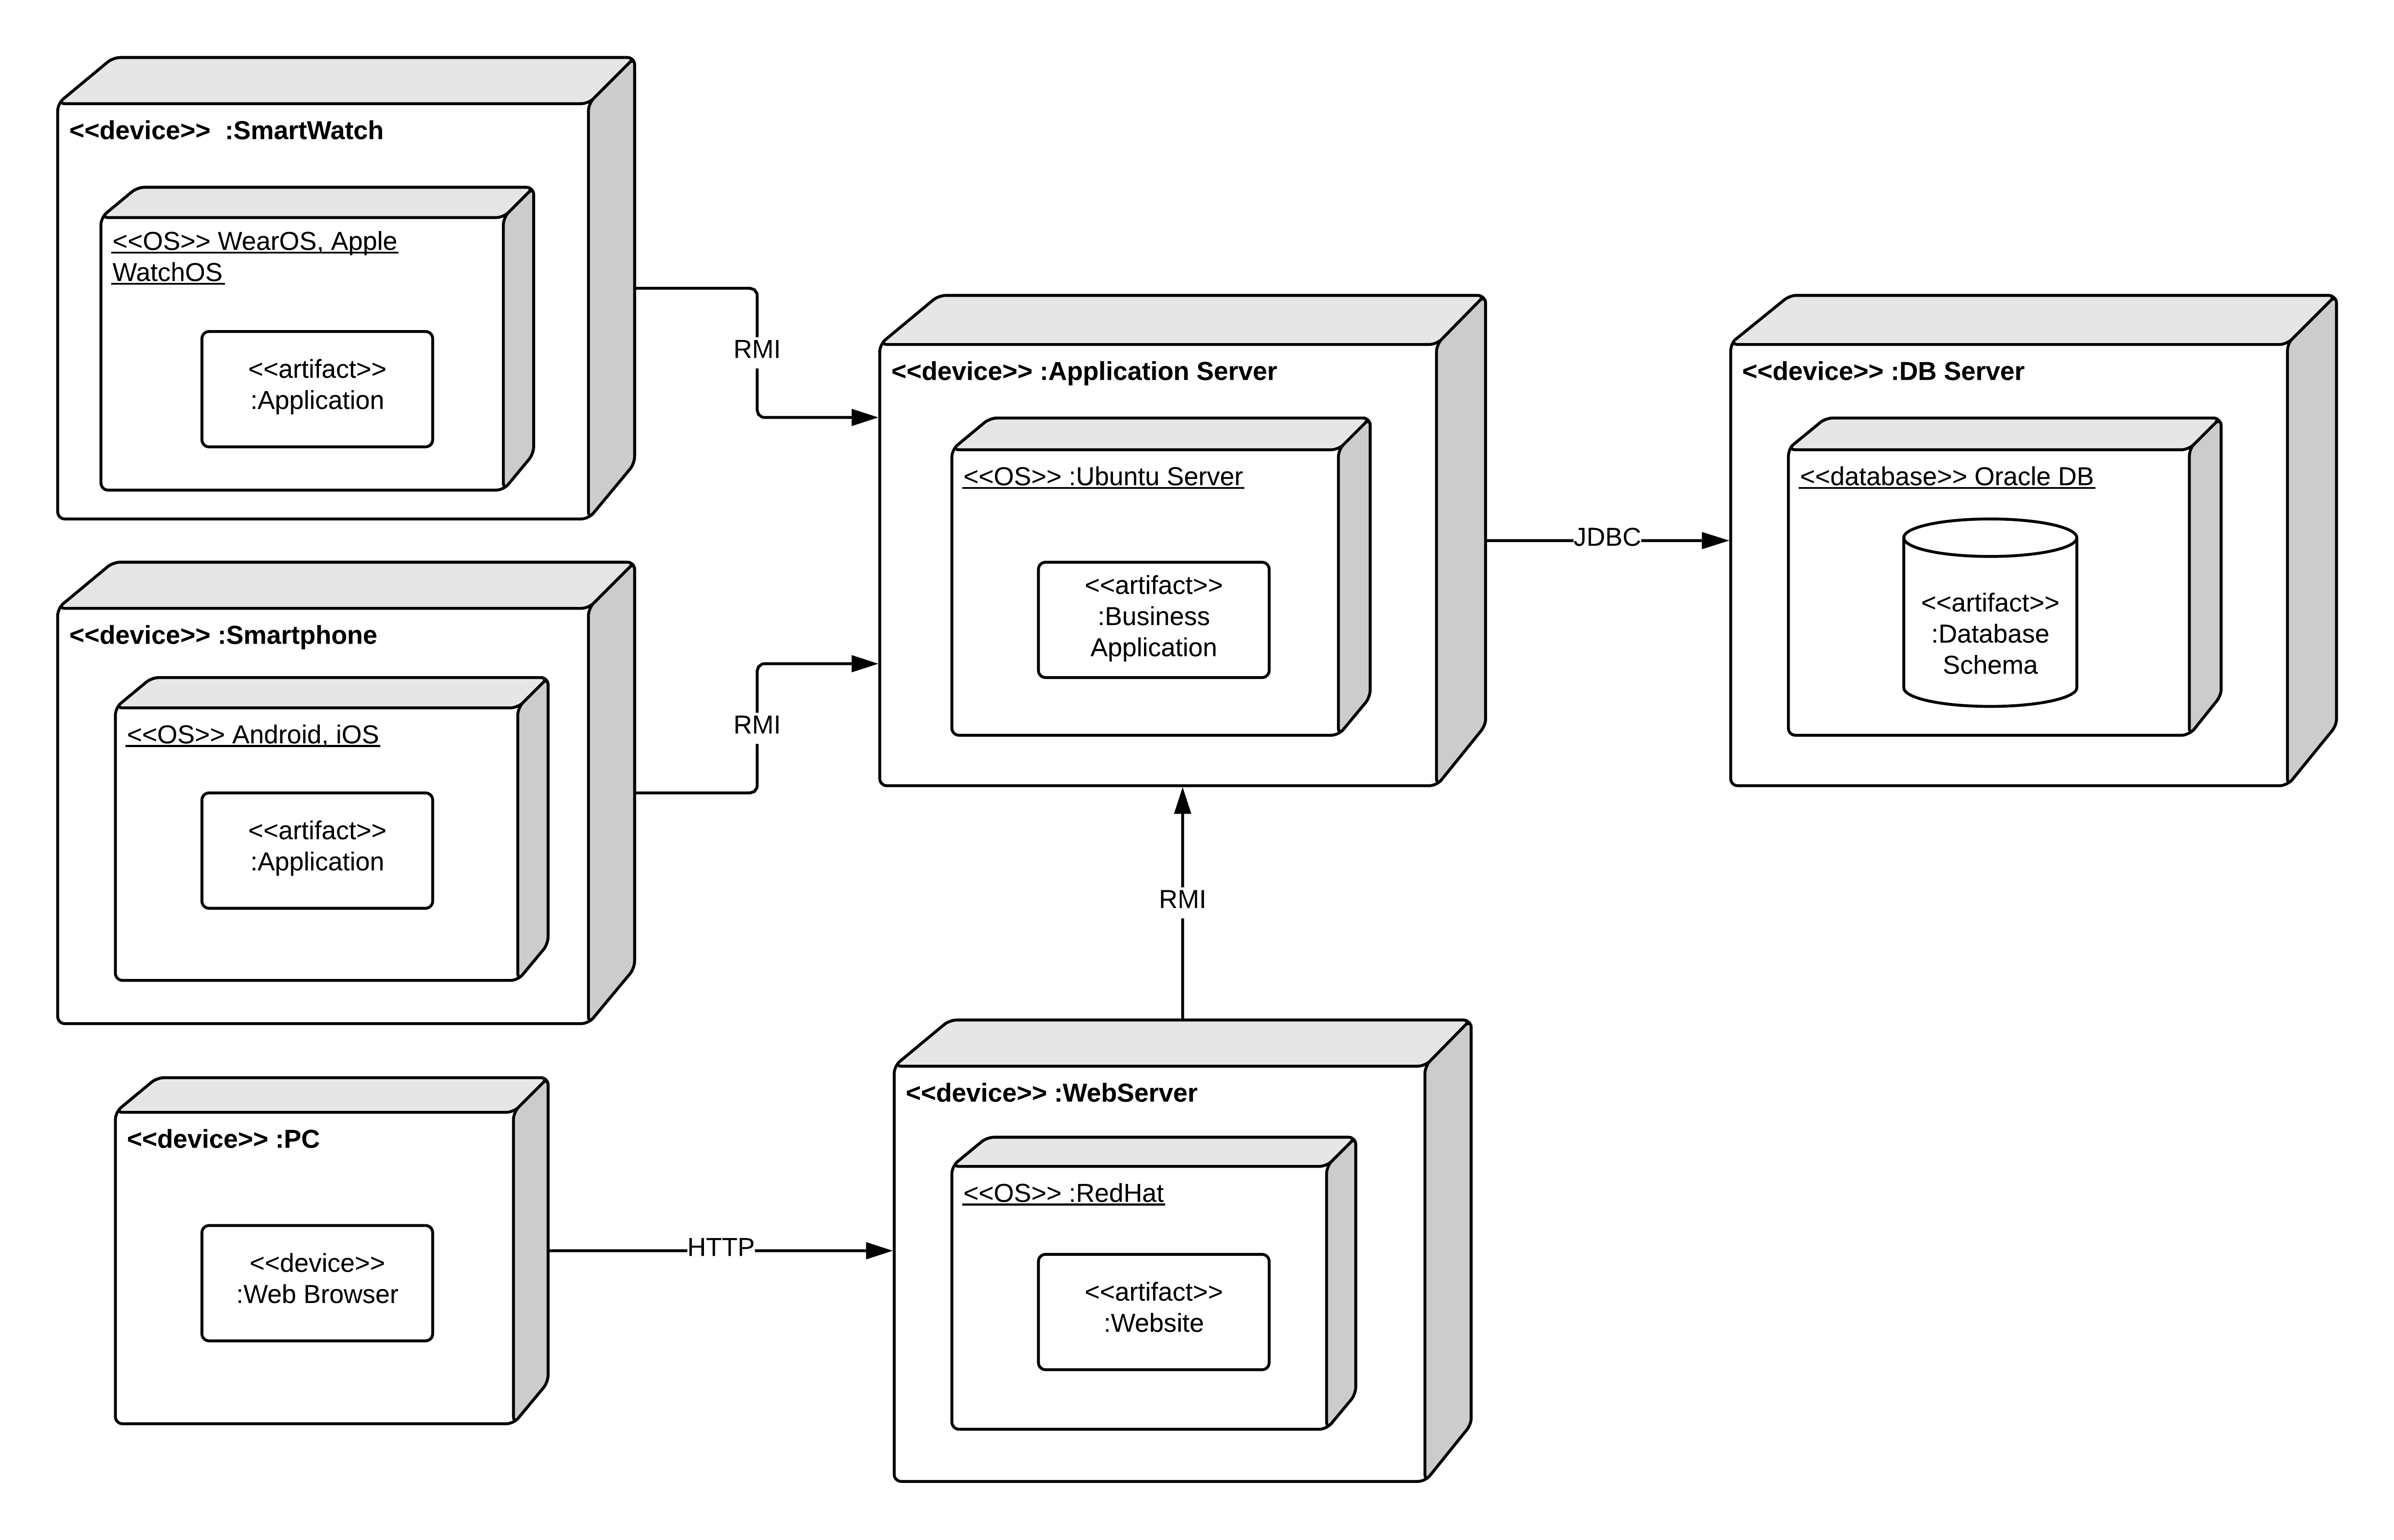
\includegraphics[scale=0.11]{Images/DeploymentDiagram.png}
\caption{Deployment Diagram}
\end{figure}
\newpage

\subsection{Runtime View}
In this section several Sequence Diagrams are shown in order to point up the interaction among components and their behavior in particular scenarios.
\subsubsection{Individual Information Request}
The following Sequence Diagram shows the interaction between components when a third party makes a request to obtain individual information. Since the individual's security number provided by the third party in the request form could not be associated to any real user (incorrect security number) or could be actually associated to a user that has not accepted the individual request privacy policy, the third party can get three different answers from the system.
\\[1.0cm]
\begin{figure}[H]
\centering
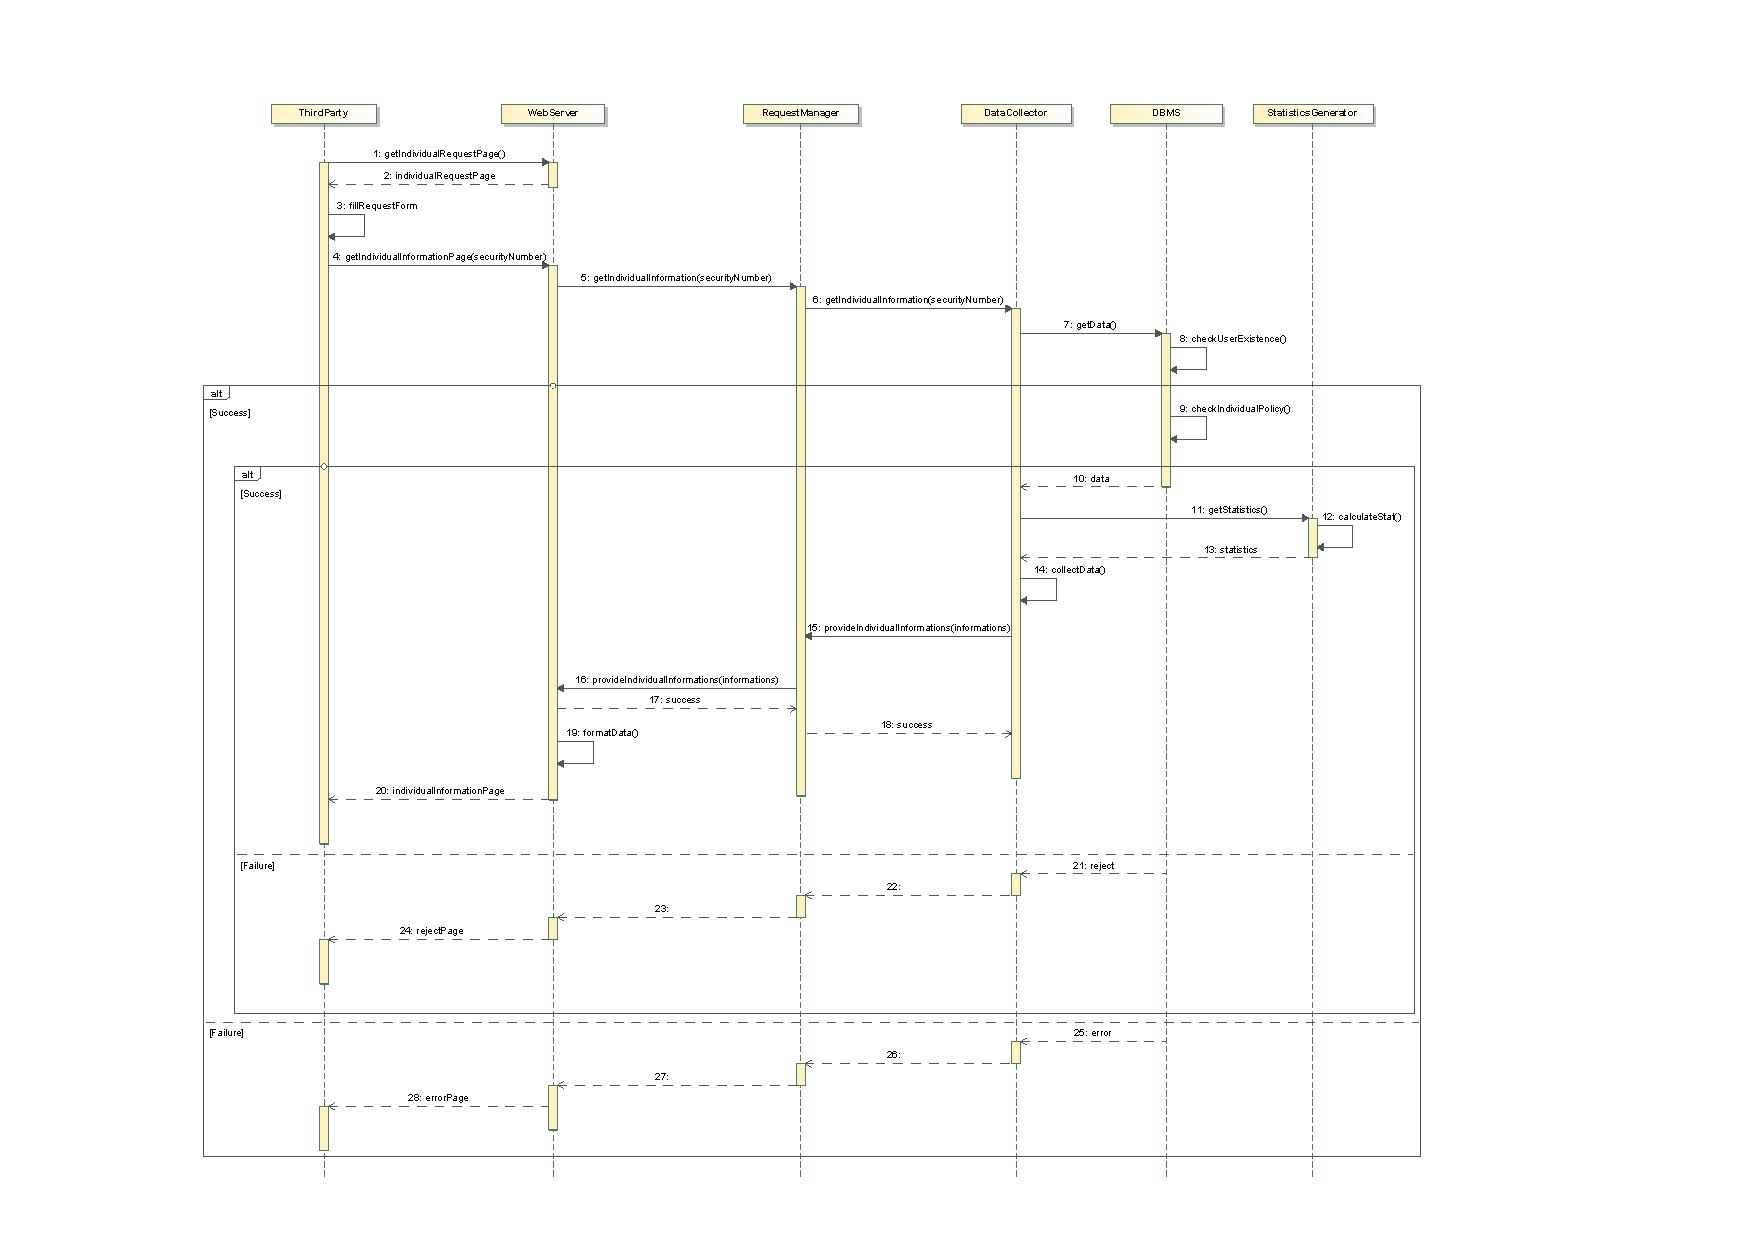
\includegraphics[scale=0.8, angle=0,origin=c]{Images/SequenceDiagrams/IndividualRequest.pdf}
\caption{Individual Information Request Sequence Diagram}
\clearpage
\end{figure}
\newpage
\subsubsection{Send Ambulance Request}
In the diagram below, the interaction between components to send an ambulance request to the first aid is shown. The data retrieved by the GPS Acquirer and HealthStatus Acquirer are both sent to Data4Help and to the HealthAnalyser.
\\[0.5cm]
\begin{figure}[H]
\centering
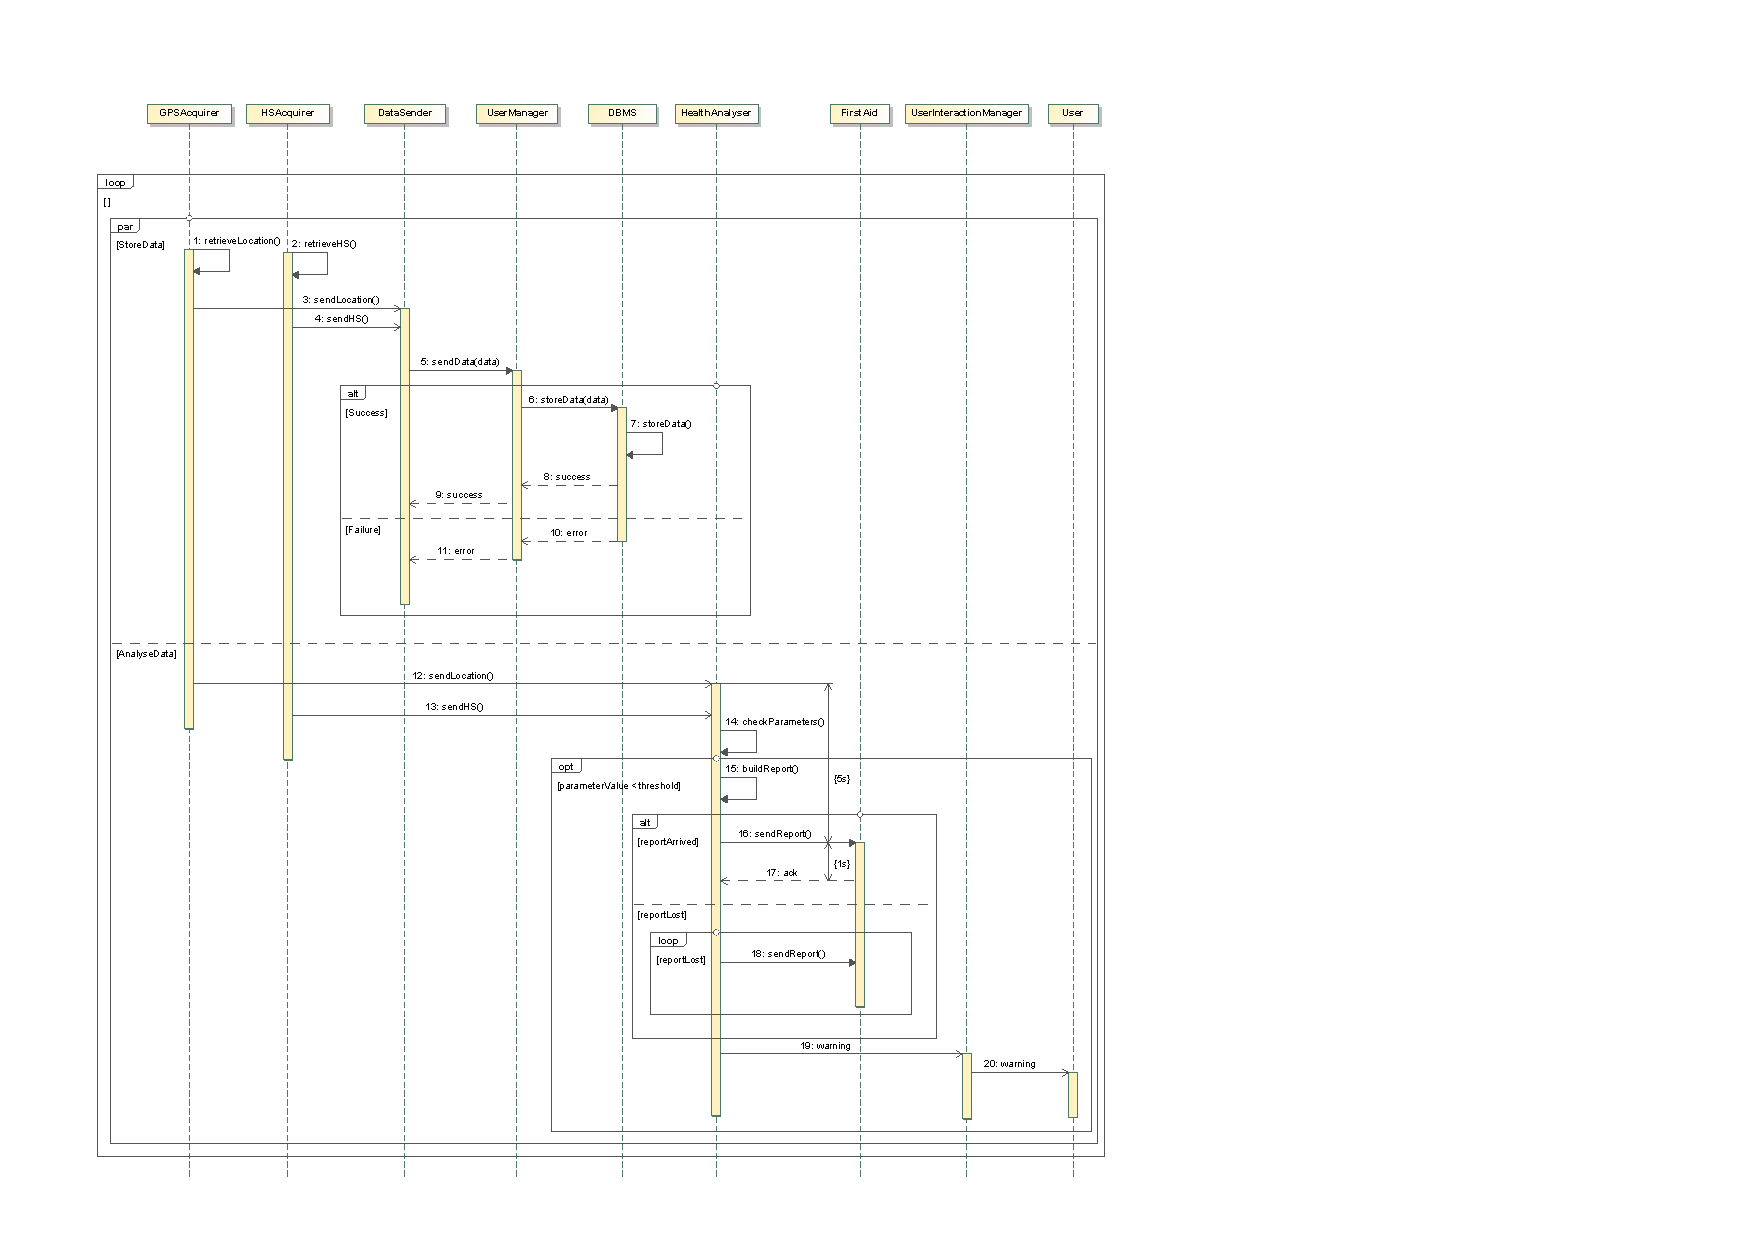
\includegraphics[scale=0.93, angle=0,origin=c]{Images/SequenceDiagrams/SendAmbulance.pdf}
\caption{Send Ambulance Request Sequence Diagram}
\clearpage
\end{figure}
\newpage
\subsubsection{Spectate A Run}
The next Sequence Diagram represents the interaction between components to show the live positions during a run event. The chart starts at the moment when the user, already logged in, select a specific run to spectate.
\\[1.0cm]
\begin{figure}[H]
\centering
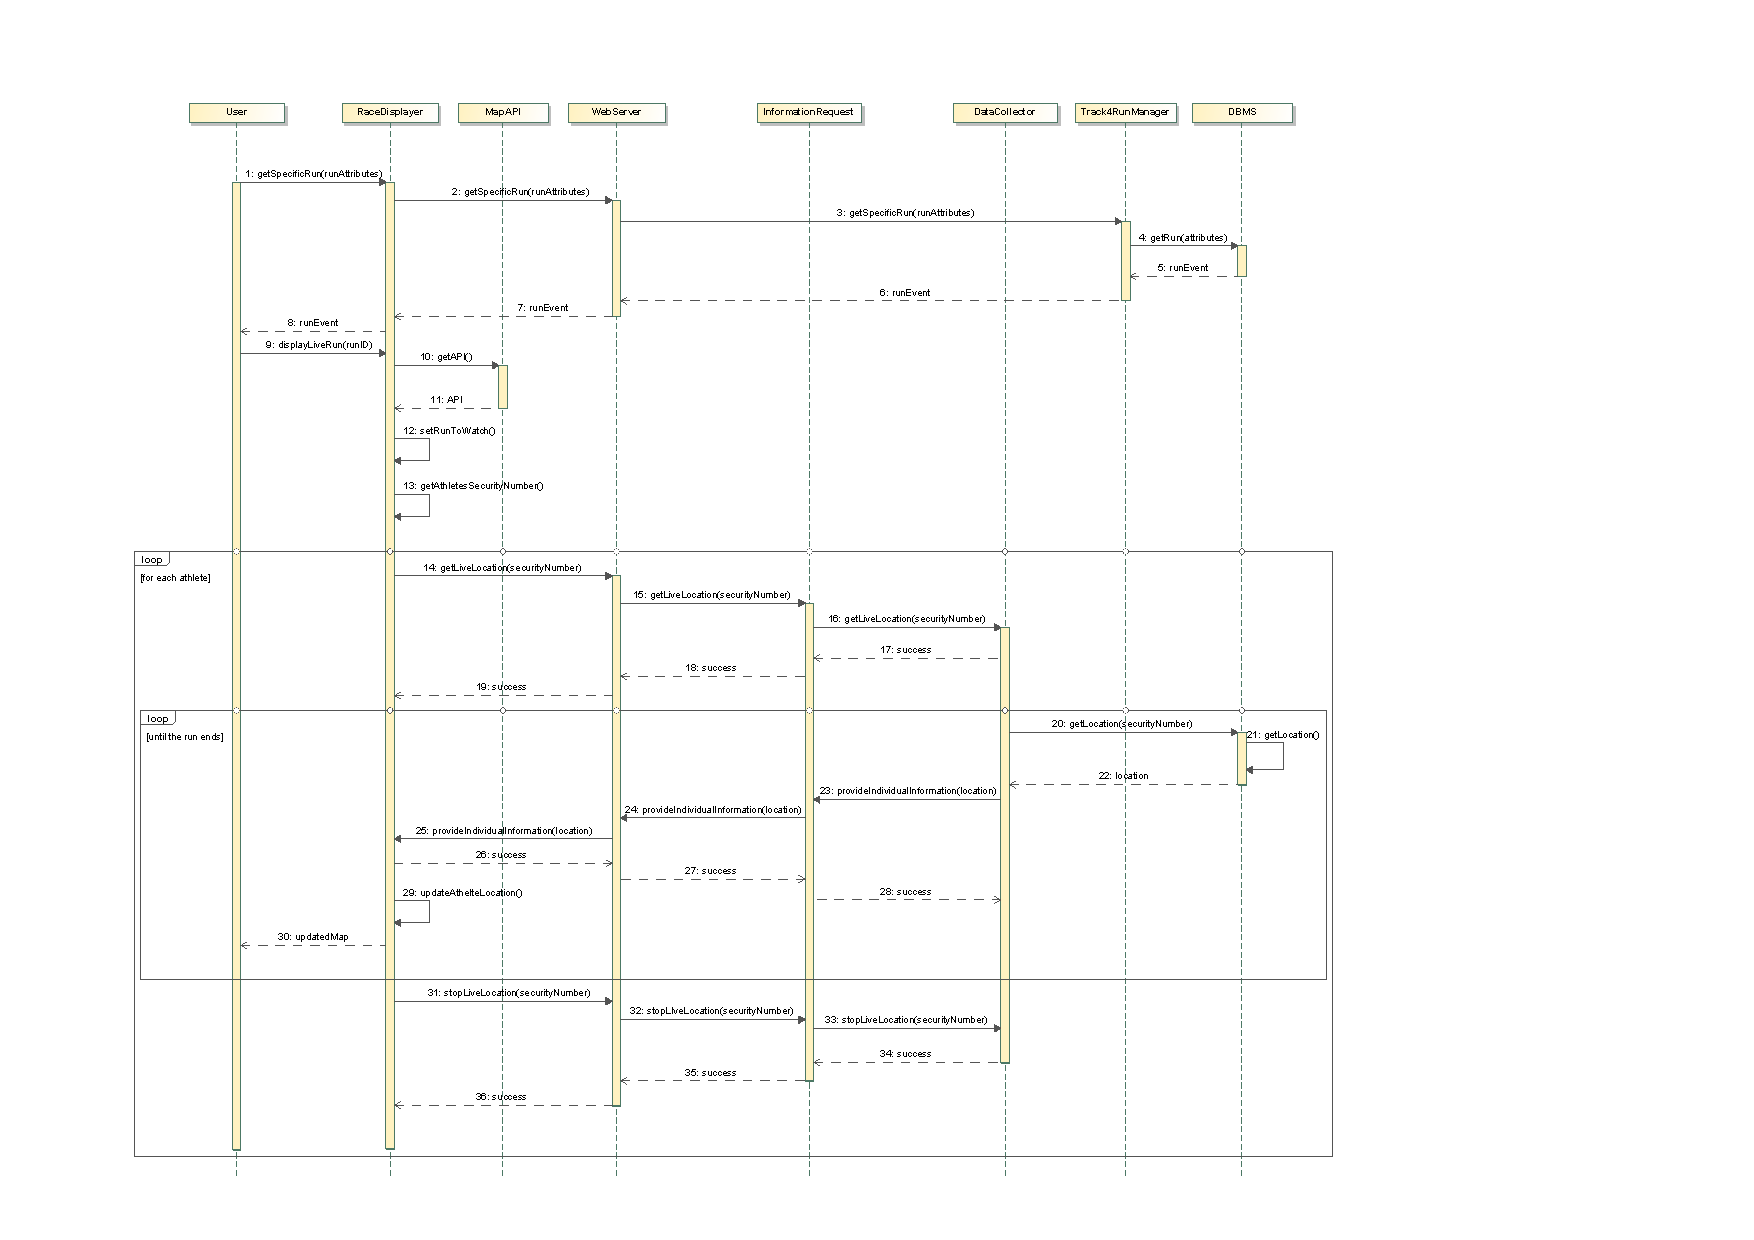
\includegraphics[scale=0.8, angle=0,origin=c]{Images/SequenceDiagrams/SpectateRun.pdf}
\caption{Spectate A Run Sequence Diagram}
\end{figure}
\clearpage


\subsection{Component Interfaces}
The following Diagram shows the dependencies between the main interfaces offered by the components of the system. In addition, for each interface it is possible to see the primary methods. 
\\[0.5cm]
\begin{figure}[H]
\centering
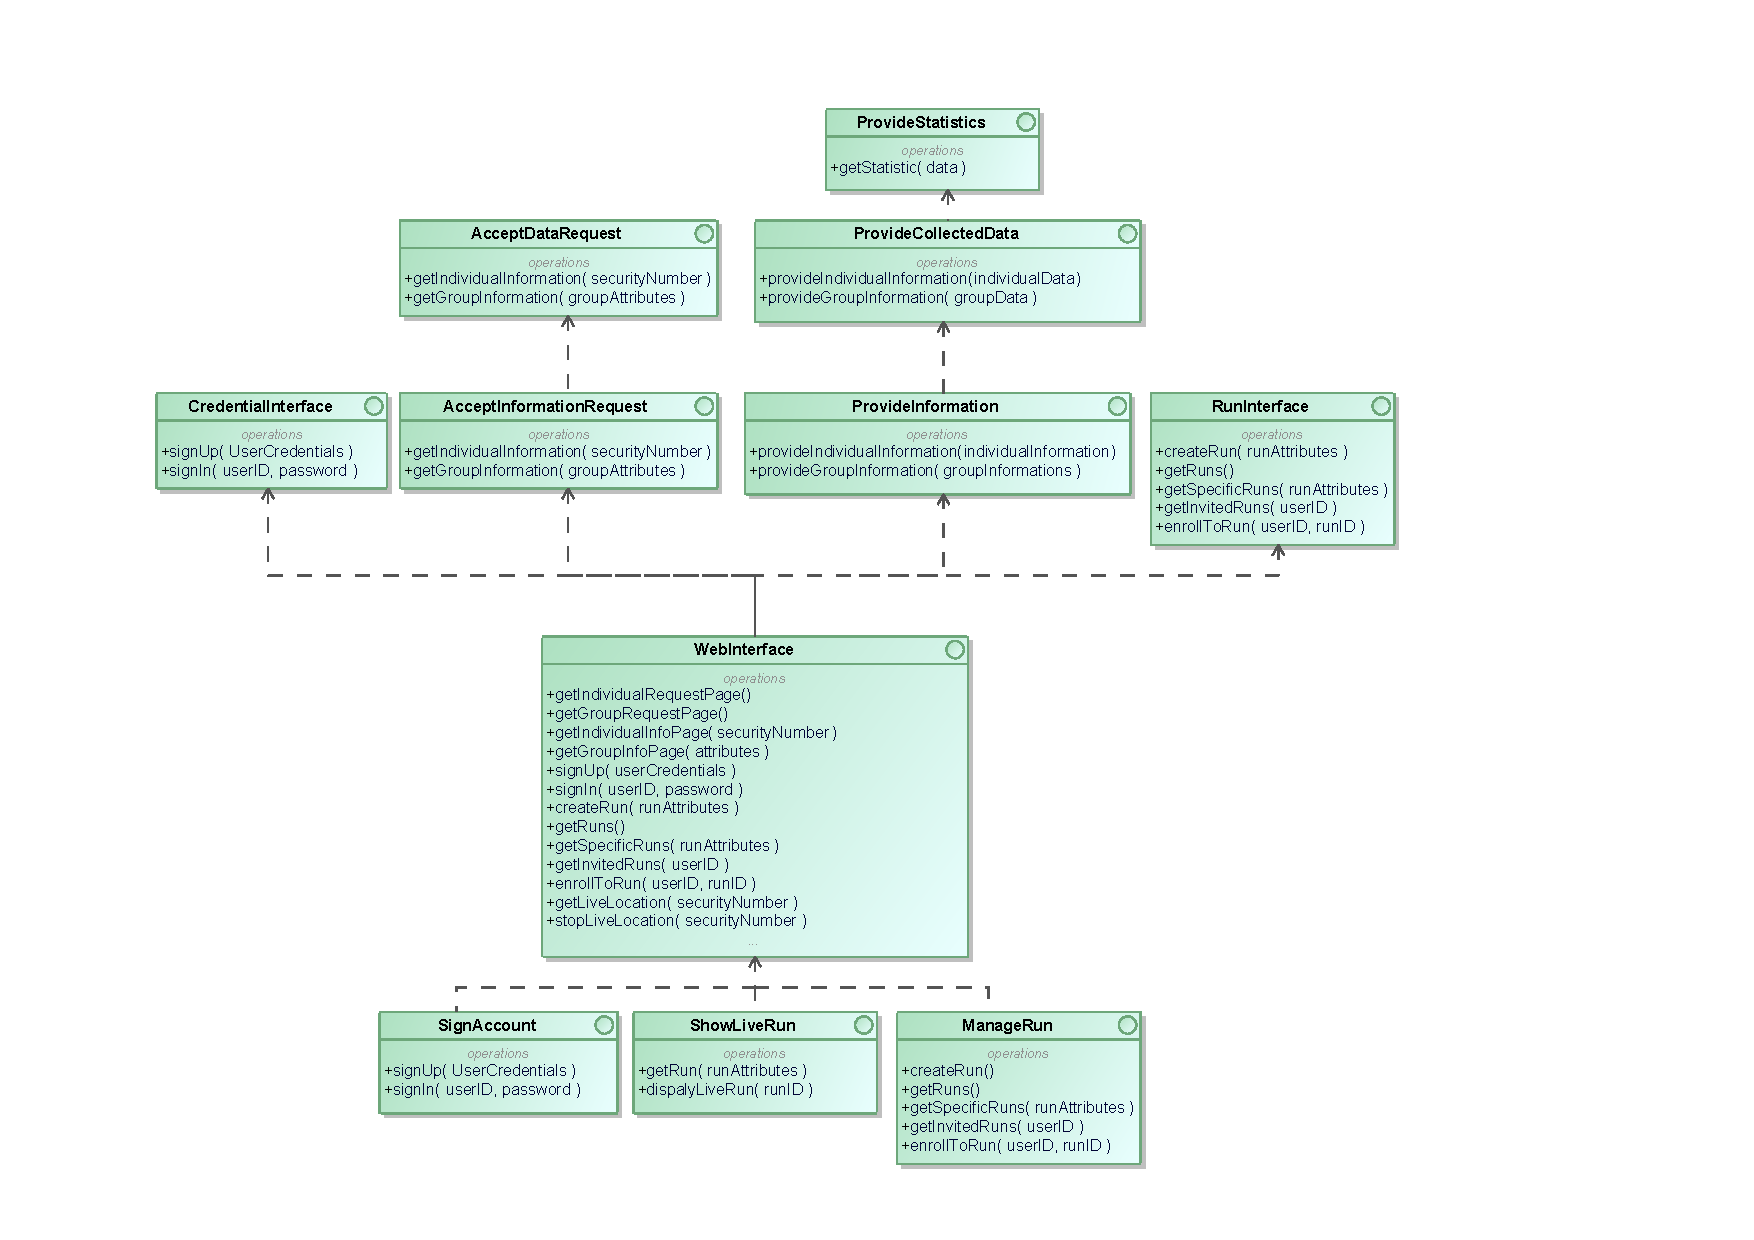
\includegraphics[scale=0.8, angle=0,origin=c]{Images/ComponentInterface.pdf}
\caption{Component Interfaces Diagram}
\end{figure}

\begin{center}
\begin{enumerate}
\item[1.1] \textbf{WebServer}
	\begin{enumerate}[nolistsep]
		\item[1.1.1] \textbf{WebInterface:} Interface for third parties that want to interact with the system in order to obtain information through Data4Help service. This interface is user also by Track4Run and AutomatedSOS in order to perform a various number of tasks.
	\end{enumerate}
	
\item[1.2] \textbf{RequestManager}
	\begin{enumerate}[nolistsep]
		\item[1.2.1] \textbf{AcceptInformationRequest:} Interface that allows the WebServer to submit requests to be evaluated.
		\item[1.2.2] \textbf{ProvideInformation:} Interface that provides to WebServer the information answers that match previous requests.
	\end{enumerate}

\item[1.3] \textbf{DataCollector}
	\begin{enumerate}[nolistsep]
		\item[1.3.1] \textbf{AcceptDataRequest:} Interface that accepts requests from the RequestManager formatted in the proper way.
		\item[1.3.2] \textbf{ProvideInformation:} Interface that provide to RequestManager the information answers formatted in the proper way.
	\end{enumerate}
	
\item[1.4] \textbf{StatisticsGenerator}
	\begin{enumerate}[nolistsep]
		\item[1.4.1] \textbf{ProvideStatistics:} Interface that provides statistics to the DataCollector.
	\end{enumerate}
	
\item[1.5] \textbf{UserDataManager}
	\begin{enumerate}[nolistsep]
		\item[1.5.1] \textbf{AcquireData:} Interface that allows partner application to send to Data4Help the acquired data.
	\end{enumerate}

\item[1.6] \textbf{Track4RunManager}
	\begin{enumerate}[nolistsep]
		\item[1.6.1] \textbf{RunInterface:} Interface that allows Track4Run application to create run events and to enroll a user to a specific run. 
	\end{enumerate}
	
\item[1.7] \textbf{CredentialsManager}
	\begin{enumerate}[nolistsep]
		\item[1.7.1] \textbf{CredentialsInterface:} Interface that saves (sign in) or checks (sign up) the credentials both from third party and individuals provided by the WebServer. Actually these operations are not performed by this interface that is only in charge of send credentials to the CredentialsManager component.
	\end{enumerate}

\item[2.1] \textbf{DBMS}
	\begin{enumerate}[nolistsep]
		\item[2.1.1] \textbf{DBInterface:} Interface that allows to store users' data into the database and to get users' data already collected in the database. This interface also allows to store and get the information about run events which are available in the database.
	\end{enumerate}
	
\item[3.1] \textbf{UserLogger}
	\begin{enumerate}[nolistsep]
		\item[3.1.1] \textbf{SignAccount:} Interface that manages sign in and sign up operations.
	\end{enumerate}
	
\item[4.1] \textbf{HealthAnalyser}
	\begin{enumerate}[nolistsep]
		\item[4.1.1] \textbf{CallAmbulance:} Software interface that allows AutomatedSOS to call, through the internet or in the worst case through telephone call, First Aid whenever is necessary in order to provide help to the user. Moreover it provides to First Aid a special report on which parameters are critical.	
	\end{enumerate}
\item[4.2] \textbf{UserInteractionManager}
	\begin{enumerate}[nolistsep]
		\item[4.2.1] \textbf{InteractionInterface:} Interface that allows the user to interact with the App, such us set the preferences, see live health status parameter values and see the (past) acquired info. This interface is also in charge of displaying the warning message on the smartwatch device.
	\end{enumerate}	
	
\item[5.1] \textbf{RunDisplayer}
	\begin{enumerate}[nolistsep]
		\item[5.1.1] \textbf{ShowLiveRun:} Interface that allows to show to the user the map in which all the athletes involved in the run are displayed.
	\end{enumerate}	

\item[5.2] \textbf{RunManager}
	\begin{enumerate}[nolistsep]
		\item[5.2.1] \textbf{ManageRun:} Interface that allows a user to create and manage a run providing all the useful information. This interface also allows a user to enroll to a run.
	\end{enumerate}		
\end{enumerate}
\clearpage
\end{center}



\subsection{Selected Architectural Styles and Patterns}

This system is designed to be a Client-Server application with three tier that well separate the different components as shown in the Overview description in order to implement the MVC software design pattern.

\begin{enumerate}
\item[•] \textbf{Architectural Design: }\\

	\begin{enumerate}
	\item[-] Client-Server architectural pattern is chosen because it is the most used and easily implemented communication pattern, in fact in our application it is the best one to supply the third parties information requests and to acquire data from users via internet. 
Regarding the acquisition of users' data, is the smartphone that decides, when data are successfully collected from the device, to call Data4Help server in order to provide and store data, furthermore even third parties call Data4Help server first and then the exchange of the information can be proceed; these two operations are the main core of the service then is logic that client-server architecture will be the right choice. 

	\item[-]Three tier architecture should be implement to assure reuse and maintainability of the system, in fact this division can permit to change some parts of the system without reconfigure the entire solution.
	
		\begin{enumerate}
		\item[*] Presentation Tier, as described above, is in charge of display on final users screen a human interface that allows the interaction with our system. This tier is present only on users' device: regarding third parties the software that is in charge to display human interface will be his own browser so the exchanged information will be an HTML page on Http connection; instead, regarding users, the software will be the application that runs on the device that works on HTML pages as well; so for both the type of users the interface to the Application Tier is the WebServer that allocate the right page to the right target. In order to supply on this aspect the partner application (AutomatedSOS and Track4Run as well) will be developed in HTML (with the support of JS and CSS) that are web languages, this aspect make also the application multi platform so they can be launched on either iOS or Android devices. Http communication protocol will be used for both connection.
		\item[*] Application Tier, as described above, is in charge to acquire all the data incoming from users, to store them on Data Tier and to handle the request on viewing data. This Tier is present on the largest part on Application server but even AutomatedSOS has inside his software an application service. All the component inside this tier will be developed in Java, in particular the Web Server runs tomcat Java servlet that generates the html pages for Presentation Tier, acquire data that users submit and communicate through RMI with the business application that runs on the Application Server. The business application is the main core of Data4Help service, and is composed by all the other components inside ApplicationServer (as Request Manager,Data Collector,Statistic Generator..); is required that it can interface with Web server, in order to acquire the external requests, and then using the components described above supply the information required; furthermore is in charge to manage all the information of users, as login or registration,or manages Track4Run races. Another very important aspect is that this application has to  retrieve data from users implementing a daemon on a specific port and listening for a TCP/IP connection incoming from partner application in order to acquire users' data. As mentioned before even AutomatedSOS implements a small part of application tier inside his software that is in charge to continuously monitor health status acquired, compare it with old data and call an ambulance via web if there is a necessity filling out a form which are indicated all the critical parameters detected.
		
	\item[*] Data Tier, as described above, is in charge to store and provide informations. This tier is present only on Database Server that is an Oracle machine using SQL schemas. The database is divided in two parts, one regarding Data4Help service that stores and manages users' data: historical users' location and health parameters; the other one regarding Track4Run that stores races' information. This Tier offers an SQL interface that can be exploit by Business application using JDBC libraries that supports SQL functions. 
		\end{enumerate}
	
	\end{enumerate}

\item[•] \textbf{Software Pattern: }

	\begin{enumerate}
	\item[-] The MVC (Model-View-Controller) is the obvious software pattern that can be applied on three tier architecture because can split the entire software solution in the three main region: the Model implements all that is described in data tier, the controller all that is described on Presentation tier and View all that is described in Presentation tier. All these 3 groups communicates each others through the so called Adapter Pattern.
	\item[-] The Adapter design pattern is developed to create an interface that permits to the MVC groups to easily communicate each others using different languages or different operating system that is mandatory in our system. This pattern is the representation of what is described on Component Interface section.
	\item[-] Strategy design pattern can be so much useful in the implementation of RequestManager component because it can dynamically change how to handle request queue in order to supply efficiently on heavy request load.
	\item[-] Proxy design pattern is an obvious consequence of Web Server, because this component stay in the middle between the two tier and creates a sort mask  that obscure what is behind it and simplify a lot the Presentation Tier software that has only to display what Web server indicates	
	\end{enumerate}

\end{enumerate}


\subsection{Other Design Decisions}